% =====================================================================
%  Podstawy teoretyczne i technologiczne — WERSJA WSTĘPNA (09.11.2026)
%  Zakres: zagadnienia P1 i P2 z listy zagadnien_do_opracowania.md,
%  bez P3 i bez punktu o absorpcji promieniowania w próbce/oknie detektora.
%  Wymaga: amsmath, siunitx (output-decimal-marker={,}), xcolor
%  Bibliografia: literatura-wstep/literatura_wstep.bib
%  Można rozbić na osobne rozdziały (np. sekcja 1 = rozdział technologiczny).
% =====================================================================
\providecommand{\TODO}[1]{\textcolor{red}{[TODO: #1]}}

\chapter{Podstawy teoretyczne i~technologiczne}
\label{ch:podstawy}

W~rozdziale opisano technologię wykonania struktur źródła elektronów,
zjawiska fizyczne wykorzystywane w~analizatorze (emisję polową,
przyspieszanie i~ogniskowanie wiązki, powstawanie promieniowania X)
oraz zasady pomiaru widma metodą EDS.

% =====================================================================
\section{Technologia wykonania struktur MEMS}
\label{sec:technologia}

\subsection{Materiały}

Podstawowymi materiałami struktury są krzem monokrystaliczny i~szkło
borokrzemowe. Stosuje się płytki krzemowe o~orientacji (100), ponieważ
w~procesie trawienia anizotropowego ściany wnęk i~otworów tworzą się
wtedy wzdłuż płaszczyzn \{111\} pod przewidywalnym kątem.
Krzem jest jednocześnie materiałem konstrukcyjnym i~przewodzącym,
dlatego wytworzone z~niego elementy mogą pełnić rolę elektrod.

Szkło borokrzemowe (np. Borofloat~33 lub Pyrex) ma współczynnik
rozszerzalności cieplnej zbliżony do krzemu (ok.
\SI{3.3e-6}{\per\kelvin} wobec ok. \SI{2.6e-6}{\per\kelvin} dla Si),
dzięki czemu połączenie krzem--szkło nie pęka po ochłodzeniu.
Zawiera ono jony sodu Na$^+$, które są niezbędne w~procesie bondingu
anodowego (p.~\ref{subsec:bonding}). Szkło służy też jako izolator
między elektrodami pracującymi przy różnych potencjałach.

\subsection{Utlenianie termiczne krzemu}

Warstwę tlenku krzemu SiO$_2$ wytwarza się przez utlenianie płytki
w~piecu w~temperaturze \SIrange{900}{1200}{\celsius}, w~atmosferze
suchego tlenu lub pary wodnej (utlenianie mokre, szybsze). Wzrost
warstwy opisuje model Deala--Grove'a. Na każdy nanometr tlenku zużywa
się ok. \SI{0.44}{\nano\metre} krzemu. Warstwa SiO$_2$ pełni rolę
maski podczas trawienia oraz izolatora elektrycznego. W~roztworach KOH
lepszą maską jest azotek krzemu Si$_3$N$_4$, który praktycznie się
w~nich nie trawi.

\subsection{Fotolitografia}

Fotolitografia przenosi wzór z~maski na powierzchnię płytki. Proces
obejmuje:
\begin{enumerate}
  \item nałożenie warstwy fotorezystu metodą wirowania,
  \item wstępne wygrzanie w~celu odparowania rozpuszczalnika,
  \item naświetlenie promieniowaniem UV przez maskę,
  \item wywołanie, czyli rozpuszczenie naświetlonych (rezyst pozytywowy)
        albo nienaświetlonych (rezyst negatywowy) obszarów,
  \item przeniesienie wzoru do warstwy maskującej (np. wytrawienie
        odsłoniętego SiO$_2$ w~buforowanym roztworze HF),
  \item usunięcie fotorezystu.
\end{enumerate}
W~strukturach źródła fotolitografia wyznacza położenie i~wymiary otworów
w~elektrodach i~membran.

\subsection{Trawienie anizotropowe krzemu w~KOH}
\label{subsec:koh}

Wodny roztwór wodorotlenku potasu (typowo \SIrange{30}{40}{\percent},
\SIrange{70}{85}{\celsius}) trawi krzem z~szybkością zależną od
orientacji krystalograficznej. Płaszczyzny (100) trawią się z~szybkością
rzędu \SI{1}{\micro\metre\per\minute}, a~płaszczyzny \{111\} wielokrotnie
wolniej (stosunek rzędu 100:1 i~więcej). W~efekcie w~płytce (100) powstają
wnęki o~ścianach nachylonych pod kątem \ang{54.74} do powierzchni,
ograniczone płaszczyznami \{111\}.

Właściwość ta jest wykorzystywana do wytwarzania:
\begin{itemize}
  \item cienkich membran (trawienie do zadanej głębokości od strony
        spodniej płytki),
  \item otworów w~elektrodach~\cite{urbanski2026phd}.
\end{itemize}
Emitera nie kształtuje się przez trawienie krzemu. Jest on płaskim
elementem krzemowym, na który nanosi się nanorurki węglowe
(p.~\ref{subsec:cnt}).
Zamiast KOH można stosować TMAH (wodorotlenek tetrametyloamoniowy), który
nie wprowadza jonów potasu, ale trawi wolniej.

\subsection{Inne metody trawienia}

Trawienie izotropowe (np. w~mieszaninie HF/HNO$_3$/CH$_3$COOH) przebiega
jednakowo we wszystkich kierunkach i~daje zaokrąglone kształty.
Trawienie suche, w~tym głębokie trawienie reaktywne jonowe DRIE (proces
Boscha), pozwala uzyskać pionowe ściany niezależnie od orientacji
kryształu, ale wymaga drogiej aparatury. Trawienie w~KOH jest tanie
i~wystarczające dla geometrii stosowanych w~źródle, dlatego jest
podstawową metodą kształtowania krzemu w~tej pracy.

\subsection{Nanoszenie emitera CNT}
\label{subsec:cnt}

Emiter elektronów wykonano z~kompozytu nanorurek węglowych
i~poliwinylopirolidonu (CNT-PVP), formowanego w~postaci mikroostrza
na podłożu emitera metodą termo-mechaniczną opracowaną w~zespole~\cite{urbanski2026phd}.
Polimer wiąże nanorurki z~podłożem, a~po uformowaniu na powierzchni
pozostaje wiele wystających końców nanorurek, które działają jako
punkty emisji. Ważnym wymaganiem jest odporność emitera na temperaturę
i~pole elektryczne występujące podczas bondingu anodowego.

W~prototypie opisanym w~tej pracy zastosowano prostszą metodę. Zawiesinę
nanorurek naniesiono mikropipetą bezpośrednio na emiter umieszczony na
płycie grzejnej nagrzanej do \SI{240}{\celsius}. Rozpuszczalnik
odparowywał w~kontakcie z~gorącym podłożem, a~nanorurki pozostawały na
powierzchni emitera w~postaci nieuporządkowanej warstwy.

\subsection{Bonding anodowy}
\label{subsec:bonding}

Bonding anodowy łączy krzem ze szkłem zawierającym jony alkaliczne.
Metodę opisali po raz pierwszy Wallis i~Pomerantz~\cite{wallis1969anodic}.
Płaskie i~czyste powierzchnie krzemu i~szkła dociska się do siebie,
podgrzewa do ok. \SIrange{300}{450}{\celsius} i~przykłada napięcie rzędu
setek woltów (krzem jako anoda). W~tej temperaturze jony Na$^+$ w~szkle
stają się ruchliwe i~przemieszczają się w~stronę katody. Przy granicy
z~krzemem pozostaje warstwa zubożona w~sód, z~nieskompensowanym ładunkiem
ujemnym jonów tlenu. Silne pole elektrostatyczne dociska powierzchnie
do kontaktu na poziomie atomowym i~powstają wiązania Si--O--Si. Złącze
jest wytrzymałe mechanicznie i~szczelne.

\paragraph{Bonding w~próżni (rozwiązanie docelowe).}
Aby wnętrze struktury było zamknięte w~próżni, ostatnie połączenie
wykonuje się w~komorze próżniowej, przy ciśnieniu rzędu
\SI{1e-5}{\hecto\pascal} lub niższym~\cite{urbanski2026phd}. Proces ten
jest trudniejszy niż bonding w~atmosferze. W~próżni nie ma przewodzenia
ciepła przez gaz, więc łączone elementy nagrzewają się słabiej niż płyta
grzejna (w~pracy~\cite{urbanski2026phd} zmierzono ok.
\SIrange{250}{300}{\celsius} przy płycie nagrzanej do
\SI{450}{\celsius}). Spada wtedy przewodność jonowa szkła i~prąd
bondingu, co prowadzi do nieszczelności. Ponadto podczas bondingu i~późniejszej pracy ze ścianek wydzielają się
gazy, dlatego w~strukturze hermetycznej potrzebny jest element
podtrzymujący próżnię, np. zintegrowana mikropompa jonowo-sorpcyjna
\cite{grzebyk2014micropump,grzebyk2017pumps}.

\paragraph{Stan obecny.}
Prototyp analizatora opisany w~tej pracy nie jest strukturą hermetyczną.
Elementy połączono bondingiem anodowym w~atmosferze, więc wnętrze
struktury nie jest zamknięte w~próżni. Badania prowadzono w~komorze
próżniowej przy ciśnieniu ok. \SI{1e-5}{\hecto\pascal}.
Hermetyzację przez bonding anodowy w~próżni przewiduje się jako
kolejny etap rozwoju przyrządu. Dla zastosowań na powierzchni ciał
pozbawionych atmosfery część wnętrza mogłaby pozostać otwarta na
naturalną próżnię otoczenia (p.~\ref{subsec:warunki}).

% =====================================================================
\section{Emisja elektronów}
\label{sec:emisja}

\subsection{Praca wyjścia i~mechanizmy emisji}

Elektrony przewodnictwa w~metalu lub półprzewodniku są utrzymywane
w~materiale przez barierę potencjału. Minimalną energię potrzebną do
wyprowadzenia elektronu z~poziomu Fermiego do próżni nazywa się pracą
wyjścia $\varphi$. Dla większości metali i~dla węgla wynosi ona
\SIrange{4}{5}{\electronvolt}. Elektron może opuścić materiał na trzy
sposoby:
\begin{itemize}
  \item \textbf{termoemisja} -- elektron uzyskuje energię większą od
        $\varphi$ dzięki wysokiej temperaturze. Gęstość prądu opisuje
        równanie Richardsona--Dushmana
        \begin{equation}
          J = A_\mathrm{G}\,T^2 \exp\!\left(-\frac{\varphi}{k_\mathrm{B}T}\right),
        \end{equation}
        gdzie $A_\mathrm{G}$ jest stałą materiałową (dla idealnego metalu
        \SI{1.2e6}{\ampere\per\metre\squared\per\kelvin\squared}).
        Katody termoemisyjne pracują w~temperaturze ok.
        \SI{2000}{\kelvin} lub wyższej i~pobierają znaczną moc
        grzania;
  \item \textbf{fotoemisja} -- energię dostarcza foton o~energii
        $h\nu > \varphi$;
  \item \textbf{emisja polowa} -- silne pole elektryczne zwęża barierę
        potencjału na tyle, że elektrony przechodzą przez nią na drodze
        tunelowania kwantowego, bez dostarczania ciepła.
\end{itemize}
W~zastosowaniach kosmicznych i~w~strukturach MEMS korzystna jest emisja
polowa: katoda nie wymaga grzania, pracuje w~temperaturze otoczenia,
a~prąd emisji można szybko zmieniać napięciem~\cite{parmee2015cntxray}.

\subsection{Emisja polowa i~równanie Fowlera--Nordheima}

Zależność gęstości prądu emisji polowej od natężenia pola $F$ na
powierzchni emitera podali Fowler i~Nordheim~\cite{fowler1928emission}.
W~uproszczonej postaci:
\begin{equation}
  J = \frac{a F^2}{\varphi}\exp\!\left(-\frac{b\,\varphi^{3/2}}{F}\right),
  \label{eq:fn}
\end{equation}
gdzie $a \approx \SI{1.54e-6}{\ampere\electronvolt\per\volt\squared}$,
$b \approx 6{,}83\cdot10^{9}\ \mathrm{eV^{-3/2}\,V\,m^{-1}}$.
Do istotnej emisji potrzebne są pola rzędu
\SIrange{1e9}{1e10}{\volt\per\metre}. Takich pól nie uzyskuje się
w~płaskim układzie elektrod przy napięciach rzędu kilowoltów, ale
powstają one lokalnie na ostrych wierzchołkach.

Wzmocnienie lokalnego pola opisuje współczynnik $\beta$:
\begin{equation}
  F = \beta\,\frac{U}{d},
\end{equation}
gdzie $U$ jest napięciem między emiterem a~elektrodą ekstrakcyjną
(bramką), a~$d$ odległością między nimi. Dla ostrza o~promieniu
wierzchołka $r$ i~wysokości $h$ współczynnik $\beta$ jest w~przybliżeniu
proporcjonalny do $h/r$. Dla nanorurek węglowych $\beta$ osiąga wartości
rzędu setek do tysięcy.

Po podstawieniu $F=\beta U/d$ do~\eqref{eq:fn} i~przemnożeniu przez
efektywną powierzchnię emisji otrzymuje się zależność prądu od napięcia,
którą zapisuje się w~postaci liniowej:
\begin{equation}
  \ln\frac{I}{U^2} = \ln C - \frac{b\,\varphi^{3/2}\,d}{\beta}\cdot\frac{1}{U}.
\end{equation}
Wykres $\ln(I/U^2)$ w~funkcji $1/U$ (wykres F--N) jest dla emisji
polowej linią prostą. Służy to do sprawdzenia, czy mierzony prąd jest
prądem emisji polowej, a~z~nachylenia prostej przy znanym $\varphi$
można wyznaczyć $\beta$.

\subsection{Nanorurki węglowe jako emitery}

Nanorurki węglowe (CNT) to zwinięte warstwy grafenu o~średnicy od ok.
\SI{1}{\nano\metre} (jednościenne) do kilkudziesięciu nanometrów
(wielościenne) i~długości do wielu mikrometrów. Jako emitery mają
kilka zalet~\cite{deheer1995cnt,milne2004cnt}:
\begin{itemize}
  \item bardzo duży stosunek długości do średnicy, a~więc duży
        współczynnik $\beta$ i~niskie napięcie progowe emisji,
  \item dobre przewodnictwo elektryczne i~cieplne,
  \item odporność chemiczną i~mechaniczną wiązań C--C, która ogranicza
        degradację wierzchołka,
  \item możliwość emisji z~wielu nanorurek jednocześnie, co daje duży
        prąd całkowity.
\end{itemize}
Pierwsze źródło elektronów z~CNT opisali de~Heer i~in. w~1995~r.
\cite{deheer1995cnt}, a~pierwsze lampy rentgenowskie z~katodą CNT
pojawiły się na początku XXI wieku
\cite{yue2002cntxray,heo2012miniature,parmee2015cntxray}. Katody CNT są
też rozważane w~układach napędu kosmicznego~\cite{huo2020cntspace}.

\subsection{Wywołanie emisji w~badanym układzie}

W~badanym układzie emisję wywołuje napięcie $U_\mathrm{B}$ przyłożone
między emiter (E) a~bramkę (B), czyli elektrodę ekstrakcyjną
z~otworem. Poniżej pewnego napięcia progowego prąd emisji jest
niemierzalny. Powyżej progu prąd rośnie wykładniczo zgodnie
z~\eqref{eq:fn}. Część elektronów trafia w~bramkę, a~część przechodzi
przez otwór i~jest przyspieszana w~stronę targetu (T) napięciem
$U_\mathrm{T}$. Prąd emisji w~obwodzie wyznaczano z~napięcia na
rezystorze \SI{100}{\kilo\ohm}, który jednocześnie ogranicza prąd
w~razie wyładowania.

\subsection{Degradacja i~niestabilność emisji}

Prąd emisji polowej jest wrażliwy na stan powierzchni emitera.
Cząsteczki gazu zaadsorbowane na wierzchołku zmieniają lokalną pracę
wyjścia, co powoduje fluktuacje prądu. Elektrony jonizują gaz resztkowy,
a~powstałe jony dodatnie są przyspieszane w~stronę emitera i~bombardują
go, co może uszkadzać nanorurki. Przy dużych prądach wierzchołki
nanorurek nagrzewają się i~mogą ulec przepaleniu. Dlatego przed pomiarami
źródło odgazowuje się przez wygrzewanie (w~tej pracy ok.
\SI{200}{\celsius}), a~pomiary prowadzi przy możliwie niskim ciśnieniu.

% =====================================================================
\section{Przyspieszanie i~ogniskowanie wiązki elektronów}
\label{sec:wiazka}

\subsection{Energia i~prędkość elektronu}

Elektron przyspieszany różnicą potencjałów $U$ uzyskuje energię
kinetyczną
\begin{equation}
  E = eU,
\end{equation}
czyli np. \SI{15}{\kilo\electronvolt} przy \SI{15}{\kilo\volt}. Prędkość
elektronu wynosi $v=\sqrt{2eU/m_e}$, co dla \SI{15}{\kilo\volt} daje
ok. \SI{7.3e7}{\metre\per\second}.

\subsection{Napięcia w~układzie}

W~układzie występują dwa napięcia o~różnych funkcjach:
\begin{itemize}
  \item \textbf{napięcie ekstrakcyjne} $U_\mathrm{B}$ (emiter--bramka)
        -- decyduje o~natężeniu pola na emiterze, a~więc o~prądzie emisji,
  \item \textbf{napięcie przyspieszające} $U_\mathrm{T}$ (emiter--target)
        -- decyduje o~energii elektronów padających na target lub próbkę,
        a~więc o~tym, które linie charakterystyczne mogą zostać wzbudzone
        (p.~\ref{subsec:jonizacja}).
\end{itemize}
Rozdzielenie tych funkcji pozwala regulować prąd wiązki niezależnie od
jej energii. W~pomiarach emisji prototypu (p.~\ref{sec:emisja-magnes})
stosowano $U_\mathrm{T}=\SI{2000}{\volt}$, a~widma rejestrowano przy
$U_\mathrm{T}=\SI{4000}{\volt}$ i~$U_\mathrm{B}=\SI{1000}{\volt}$.
Energia elektronów padających na target wynosiła więc podczas rejestracji widm
\SI{4}{\kilo\electronvolt}, co potwierdza granica widma ciągłego przy
ok. \SI{4}{\kilo\electronvolt}. W~obwodzie mierzy się prąd bramki i~prąd targetu. Ich
różnica względem prądu emisji wskazuje na prądy upływu lub elektrony
docierające do innych elementów.

\subsection{Ruch elektronu w~polu magnetycznym}

Na elektron poruszający się w~polu elektrycznym $\vec{E}$ i~magnetycznym
$\vec{B}$ działa siła Lorentza
\begin{equation}
  \vec{F} = -e\left(\vec{E} + \vec{v}\times\vec{B}\right).
\end{equation}
Składowa prędkości równoległa do linii pola magnetycznego nie zmienia
się, a~składowa prostopadła $v_\perp$ powoduje ruch po okręgu
o~promieniu Larmora
\begin{equation}
  r_\mathrm{L} = \frac{m_e v_\perp}{eB}.
\end{equation}
Wypadkowy ruch to spirala nawinięta na linię pola. Elektrony wylatujące
z~emitera pod różnymi kątami są więc utrzymywane w~pobliżu linii pola
przechodzących przez emiter, zamiast rozbiegać się na boki. Przy indukcji
rzędu \SI{0.1}{\tesla} i~składowej poprzecznej energii rzędu
\SI{10}{\electronvolt} promień Larmora wynosi ok.
\SI{0.1}{\milli\metre}.

\subsection{Ogniskowanie magnetyczne}

Pole magnetyczne o~symetrii osiowej działa na wiązkę elektronów jak
soczewka skupiająca. W~przybliżeniu cienkiej soczewki jej ogniskową
opisuje wzór Buscha
\begin{equation}
  \frac{1}{f} = \frac{e}{8 m_e U}\int B_z^2(z)\,\mathrm{d}z,
\end{equation}
z~którego wynika, że ogniskowanie jest tym silniejsze, im większa jest
indukcja i~im mniejsza energia elektronów~\cite{goldstein2018sem}.
W~mikroskopach elektronowych stosuje się elektromagnesy z~nabiegunnikami.
W~miniaturowym źródle zastosowano prosty magnes trwały NdFeB umieszczony
pod katodą z~emiterem, a~w~badanym prototypie magnes umieszczono na
emiterze. Parametrów tego magnesu (indukcji, wymiarów) nie mierzono,
dlatego jego działanie oceniano tylko na podstawie prądu i~obrazu
wiązki. Elektrony podążają wzdłuż jego linii pola, co
poprawia skupienie i~jednorodność wiązki w~porównaniu z~samym
ogniskowaniem elektrostatycznym~\cite{urbanski2026phd,grzebyk2017magnetic}.
W~pomiarach wykonanych w~tej pracy z~magnesem obserwowano zwartą plamkę
na ekranie zamiast oświetlenia całego okna; wpływu magnesu na prąd nie
dało się oddzielić od stanu powierzchni emitera
(p.~\ref{sec:emisja-magnes}).

\subsection{Ogniskowanie elektrostatyczne}

Wiązkę można też ogniskować polem elektrycznym elektrod o~odpowiednio
ukształtowanych otworach (soczewki elektrostatyczne, np. pojedyncza
soczewka Einzela). W~strukturach MEMS elektrody takie wykonuje się
z~krzemu, ale ich wymiary i~odległości są ograniczone grubością płytek,
a~ich ustawienie względem siebie musi być bardzo dokładne. W~pracy
\cite{urbanski2026phd} samo ogniskowanie elektrostatyczne okazało się
niewystarczające, co uzasadnia użycie magnesu.

\subsection{Obserwacja wiązki na ekranie luminescencyjnym}

Kształt i~położenie wiązki obserwuje się na ekranie pokrytym luminoforem,
który świeci w~miejscu padania elektronów. Jasność świecenia rośnie
z~gęstością prądu, dlatego zdjęcie ekranu pokazuje rozkład gęstości
prądu w~przekroju wiązki. Metoda ta jest jakościowa: jasność zależy też
od energii elektronów, rodzaju luminoforu, jego degradacji i~ustawień
aparatu.

% =====================================================================
\section{Powstawanie promieniowania X}
\label{sec:rtg}

\subsection{Oddziaływanie elektronów z~materią}

Elektron wnikający w~materiał ulega rozpraszaniu sprężystemu (na
jądrach, zmiana kierunku bez straty energii) i~niesprężystemu (na
elektronach atomów, strata energii). Wypadkowa trajektoria jest
zygzakowata, a~obszar, w~którym zachodzą oddziaływania, ma kształt
gruszki lub półkuli pod punktem padania wiązki. Produktami oddziaływań
są elektrony wtórne, elektrony wstecznie rozproszone, ciepło oraz
promieniowanie X: ciągłe i~charakterystyczne~\cite{goldstein2018sem}.

Głębokość wnikania elektronów opisuje zasięg Kanayi--Okayamy
\begin{equation}
  R\,[\si{\micro\metre}] = \frac{0{,}0276\,A\,E_0^{1{,}67}}{Z^{0{,}89}\,\rho},
\end{equation}
gdzie $A$ -- masa atomowa [g/mol], $E_0$ -- energia elektronów [keV],
$Z$ -- liczba atomowa, $\rho$ -- gęstość [g/cm$^3$]. Dla krzemu przy
\SI{15}{\kilo\electronvolt} zasięg wynosi ok. \SI{3}{\micro\metre}.
Analiza EDS dotyczy więc warstwy przypowierzchniowej próbki o~grubości
rzędu mikrometrów.

\subsection{Promieniowanie hamowania}

Elektron hamowany w~polu elektrycznym jądra traci część energii, która
jest emitowana jako foton. Ponieważ strata energii w~pojedynczym
zdarzeniu może mieć dowolną wartość od zera do całej energii elektronu,
widmo promieniowania hamowania (\emph{bremsstrahlung}) jest ciągłe.
Kształt widma opisuje w~przybliżeniu wzór Kramersa
\begin{equation}
  N(E) \approx k\,i\,Z\,\frac{E_0-E}{E},
\end{equation}
gdzie $N(E)$ jest liczbą fotonów o~energii $E$ w~jednostkowym przedziale
energii, $i$ -- prądem wiązki, $k$ -- stałą. Widmo kończy się na
energii równej energii elektronów (granica Duane'a--Hunta):
\begin{equation}
  E_\mathrm{max} = eU, \qquad
  \lambda_\mathrm{min}\,[\si{\nano\metre}] = \frac{1{,}2398}{U\,[\si{\kilo\volt}]}.
\end{equation}
W~analizie EDS promieniowanie hamowania stanowi tło, na którym widoczne
są linie charakterystyczne. Pomiar granicy Duane'a--Hunta w~widmie pozwala
sprawdzić rzeczywistą energię elektronów docierających do próbki. Kształt widma dla dwóch energii elektronów przedstawiono na
rys.~\ref{fig:kramers}.

\begin{figure}[htbp]
  \centering
  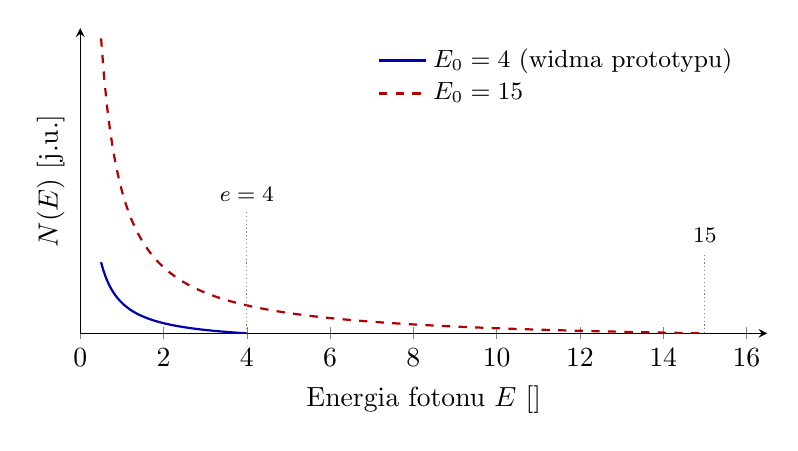
\begin{tikzpicture}
    \begin{axis}[
        width=0.85\linewidth, height=0.45\linewidth,
        xmin=0, xmax=16.5, ymin=0, ymax=30,
        xlabel={Energia fotonu $E$ [\si{\kilo\electronvolt}]},
        ylabel={$N(E)$ [j.u.]},
        ytick=\empty, axis lines=left,
        legend style={draw=none, font=\small}, legend cell align=left, legend pos=north east]
      \addplot[thick, blue!70!black, domain=0.5:4, samples=120]
        {(4-x)/x};
      \addlegendentry{$E_0=\SI{4}{\kilo\electronvolt}$ (widma prototypu)}
      \addplot[thick, red!70!black, dashed, domain=0.5:15, samples=200]
        {(15-x)/x};
      \addlegendentry{$E_0=\SI{15}{\kilo\electronvolt}$}
      \draw[gray, densely dotted] (axis cs:4,0) -- (axis cs:4,12)
        node[above, font=\footnotesize, black] {$e\UT=\SI{4}{\kilo\electronvolt}$};
      \draw[gray, densely dotted] (axis cs:15,0) -- (axis cs:15,8)
        node[above, font=\footnotesize, black] {\SI{15}{\kilo\electronvolt}};
    \end{axis}
  \end{tikzpicture}
  \caption{Widmo promieniowania hamowania według wzoru Kramersa dla dwóch
    energii elektronów; widmo kończy się na granicy Duane'a--Hunta
    $E_\mathrm{max}=eU$. Na widmo ciągłe nakładają się linie
    charakterystyczne, a~przy małych energiach jest ono osłabiane przez
    absorpcję w~próbce i~oknie detektora \opracowanieWlasne}
  \label{fig:kramers}
\end{figure}

\subsection{Jonizacja powłok wewnętrznych}
\label{subsec:jonizacja}

Elektron wiązki może wybić elektron z~wewnętrznej powłoki atomu (K, L,
M), jeśli jego energia jest większa od energii wiązania tej powłoki,
nazywanej energią krytyczną $E_\mathrm{c}$ (odpowiada ona krawędzi
absorpcji). Na przykład dla powłoki K krzemu
$E_\mathrm{c}=\SI{1.84}{\kilo\electronvolt}$, a~dla żelaza
\SI{7.11}{\kilo\electronvolt}. Stosunek energii elektronów do energii
krytycznej nazywa się współczynnikiem nadnapięcia
\begin{equation}
  U_0 = \frac{E_0}{E_\mathrm{c}}.
\end{equation}
Natężenie linii charakterystycznej rośnie w~przybliżeniu jak
$(U_0-1)^{n}$, gdzie $n\approx1{,}5$--$1{,}7$. W~praktyce do skutecznego
wzbudzenia linii stosuje się $U_0\approx2$--3. Przy napięciu
przyspieszającym \SI{15}{\kilo\volt} dobrze wzbudzane są linie K
pierwiastków do żelaza włącznie, co obejmuje główne pierwiastki
skałotwórcze (O, Mg, Al, Si, Ca, Fe). Przy energii
\SI{4}{\kilo\electronvolt}, stosowanej przy rejestracji widm prototypu,
warunek $U_0\geq2$ spełniają linie K pierwiastków o~energii krytycznej do
ok. \SI{2}{\kilo\electronvolt}: O, Na, Mg, Al i~Si. Linie K fosforu
i~siarki są wzbudzane słabiej ($U_0\approx1{,}6$--1{,}9), linia K potasu
tylko śladowo, a~linii K wapnia ($E_\mathrm{c}=\SI{4.04}{\kilo\electronvolt}$)
i~linii K żelaza ($E_\mathrm{c}=\SI{7.11}{\kilo\electronvolt}$) nie da się wzbudzić.
Żelazo i~inne metale przejściowe można wtedy rozpoznać tylko po liniach L
(np. Fe L$\alpha$ \SI{0.705}{\kilo\electronvolt}). Pomiary emisji przy
$U_\mathrm{T}=\SI{2}{\kilo\volt}$ służyły do badania źródła elektronów,
a~nie do analizy widma.

\subsection{Relaksacja atomu i~emisja fotonu promieniowania X}

Po jonizacji powłoki wewnętrznej atom znajduje się w~stanie wzbudzonym.
Lukę zapełnia elektron z~wyższej powłoki, a~nadmiar energii, równy
różnicy energii wiązania obu powłok, zostaje wypromieniowany jako foton
promieniowania X. Energie powłok są inne dla każdego pierwiastka, dlatego
energia fotonu jest cechą charakterystyczną pierwiastka i~na niej opiera
się identyfikacja składu w~spektroskopii EDS. Przykładowo przejście
elektronu z~powłoki L na powłokę K w~atomie glinu daje foton Al~\Ka{}
o~energii \SI{1.486}{\kilo\electronvolt}.

Nie każda relaksacja kończy się emisją fotonu. W~konkurencyjnym efekcie
Augera nadmiar energii przejmuje inny elektron atomu, który opuszcza atom,
i~foton nie powstaje. Udział relaksacji z~emisją fotonu opisuje wydajność
fluorescencji $\omega$, rosnąca z~liczbą atomową: dla powłoki K krzemu
wynosi ok.~\num{0.05}, a~dla żelaza ok.~\num{0.35}. Lekkie pierwiastki
emitują więc mniej fotonów na jedną jonizację i~dają w~widmie słabsze
linie~\cite{goldstein2018sem,beckhoff2006xrf}.

\subsection{Nazewnictwo linii i~prawo Moseleya}

Linie oznacza się literą powłoki, na której powstała luka, oraz
indeksem określającym, skąd pochodzi elektron zapełniający:
K$\alpha$ (przejście L$\to$K), K$\beta$ (M$\to$K), L$\alpha$ (M$\to$L)
itd. (notacja Siegbahna; w~notacji IUPAC np. K$\alpha_1$ = K--L$_3$).
Energia linii zależy od liczby atomowej zgodnie z~prawem Moseleya.
Dla linii K$\alpha$ w~przybliżeniu
\begin{equation}
  E_{\mathrm{K}\alpha} \approx \SI{10.2}{\electronvolt}\,(Z-1)^2,
\end{equation}
co np. dla żelaza ($Z=26$) daje ok. \SI{6.4}{\kilo\electronvolt},
zgodnie z~wartością tablicową. Jednoznaczna zależność energii linii od
$Z$ jest podstawą identyfikacji pierwiastków w~widmie.
Przykładowe energie linii K$\alpha$: O~\SI{0.525}{\kilo\electronvolt},
Mg \SI{1.254}{\kilo\electronvolt}, Al \SI{1.487}{\kilo\electronvolt},
Si \SI{1.740}{\kilo\electronvolt}, Ca \SI{3.69}{\kilo\electronvolt},
Fe \SI{6.40}{\kilo\electronvolt}.

\subsection{EDS a~XRF}

Obie metody rejestrują to samo promieniowanie charakterystyczne, ale
różnią się sposobem wzbudzenia:
\begin{itemize}
  \item w~\textbf{EDS} (w~mikroskopie elektronowym) próbkę wzbudza wiązka
        elektronów. Wiązkę łatwo zogniskować do małej plamki
        i~wydajnie wzbudza ona pierwiastki lekkie, ale towarzyszy jej
        silne tło promieniowania hamowania, a~próbka nieprzewodząca może
        się ładować;
  \item w~\textbf{XRF} próbkę wzbudzają fotony promieniowania X (z~lampy
        rentgenowskiej lub izotopu). Tło jest znacznie mniejsze, bo nie
        powstaje promieniowanie hamowania w~próbce, ale wzbudzenie
        pierwiastków lekkich jest słabsze, a~ogniskowanie promieniowania
        X wymaga specjalnej optyki~\cite{beckhoff2006xrf}.
\end{itemize}
Miniaturowe źródło RTG MEMS rozwijane na Politechnice Wrocławskiej
zastosowano dotychczas do spektrometrii XRF~\cite{urbanski2026xrf}.
W~tej pracy wiązka elektronów pada bezpośrednio na próbkę, czyli
przyrząd działa jak analizator EDS.

\subsection{Target transmisyjny i~odbiciowy}
\label{subsec:target}

W~źródle rentgenowskim wiązka elektronów pada na target. W~targecie
odbiciowym promieniowanie wyprowadza się od strony padania wiązki, pod
kątem do jej osi. W~targecie transmisyjnym warstwa metalu (np. W, Mo)
jest naniesiona na cienką membranę, a~promieniowanie wychodzi na wylot,
wzdłuż osi wiązki. Grubość warstwy dobiera się tak, aby była porównywalna
z~zasięgiem elektronów: zbyt cienka nie wykorzysta energii wiązki, zbyt
gruba pochłonie wytworzone promieniowanie. Konstrukcja transmisyjna
pozwala zbudować źródło osiowe i~zwarte, dlatego zastosowano ją w~źródle
MEMS~\cite{urbanski2023target,urbanski2024monochromatic}. W~analizatorze
EDS rolę targetu pełni badana próbka.

% =====================================================================
\section{Pomiar widma metodą EDS}
\label{sec:spektrometria}

\subsection{Stanowisko pomiarowe}

Stanowisko składa się z~komory próżniowej z~układem pomp, badanej
struktury (emiter, bramka, target lub próbka), dwóch zasilaczy
wysokiego napięcia (obwód bramki i~obwód targetu), rezystorów
ograniczających \SI{100}{\kilo\ohm} z~woltomierzami do pomiaru prądów
oraz spektrometru rentgenowskiego ustawionego tak, aby widział
oświetlany obszar próbki. Ciśnienie w~komorze podczas pomiarów wynosiło
ok. \SI{1e-5}{\hecto\pascal}. Charakterystyki emisji mierzono przy
$U_\mathrm{T}=\SI{2000}{\volt}$, a~widma przy
$U_\mathrm{T}=\SI{4000}{\volt}$ i~$U_\mathrm{B}=\SI{1000}{\volt}$.
Schemat elektryczny przedstawiono na rys.~\ref{fig:uklad-pomiarowy}.

\subsection{Charakterystyka prądowo-napięciowa emitera}

Podstawowym pomiarem źródła elektronów jest zależność prądu emisji od
napięcia bramki $I(U_\mathrm{B})$ przy stałym $U_\mathrm{T}$.
Z~charakterystyki odczytuje się napięcie progowe i~maksymalny stabilny
prąd. Wykres F--N służy do potwierdzenia mechanizmu emisji. Pomiary
porównawcze z~magnesem i~bez magnesu oraz przed i~po odgazowaniu
pokazują wpływ ogniskowania i~stanu powierzchni emitera.

\subsection{Półprzewodnikowy detektor promieniowania X}

Foton promieniowania X pochłonięty w~krysztale półprzewodnika wytwarza
pary elektron--dziura. Średnia energia na wytworzenie jednej pary
w~krzemie wynosi $\varepsilon\approx\SI{3.6}{\electronvolt}$, więc foton
o~energii \SI{6}{\kilo\electronvolt} wytwarza ok. 1600 par. Pole
elektryczne w~detektorze rozdziela nośniki, zanim zdążą zrekombinować,
i~zbiera je na elektrodach. Zebrany ładunek jest proporcjonalny do
energii fotonu~\cite{urbanski2023detection}.

Stosowane typy detektorów:
\begin{itemize}
  \item \textbf{Si(Li)} -- krzem kompensowany litem, wymaga chłodzenia
        ciekłym azotem,
  \item \textbf{SDD} (krzemowy detektor dryfowy) -- elektrony dryfują do
        małej anody o~niskiej pojemności, co obniża szumy i~pozwala na
        duże szybkości zliczeń. Chłodzony ogniwem Peltiera, obecnie
        najczęściej stosowany,
  \item \textbf{CdTe} -- wyższa liczba atomowa, lepsza wydajność dla
        energii powyżej ok. \SI{20}{\kilo\electronvolt}, gorsza
        rozdzielczość.
\end{itemize}
Typ detektora w~spektrometrze użytym do pomiarów nie był znany, dlatego
w~pracy opisano zasadę działania detektorów półprzewodnikowych ogólnie.

\subsection{Tor akwizycji}

Ładunek z~detektora jest zamieniany na impuls napięciowy przez
przedwzmacniacz ładunkowy. Układ kształtujący (obecnie cyfrowy procesor
impulsów) filtruje sygnał i~mierzy amplitudę każdego impulsu.
Analizator wielokanałowy (MCA) przypisuje impuls do kanału odpowiadającego
jego amplitudzie i~zlicza impulsy w~kanałach. Wynikiem jest histogram
liczby zliczeń w~funkcji energii, czyli widmo.

\subsection{Analiza widma}

Analiza jakościowa polega na przypisaniu pikom pierwiastków na
podstawie energii linii. Należy uwzględnić zjawiska, które dają piki
pozorne lub zniekształcenia:
\begin{itemize}
  \item \textbf{tło promieniowania hamowania}, które trzeba odjąć przed
        wyznaczeniem pola powierzchni pików,
  \item \textbf{piki ucieczki} -- foton padający wzbudza w~detektorze
        krzemowym promieniowanie Si K$\alpha$, które ucieka z~kryształu.
        Rejestrowana jest wtedy energia mniejsza o~\SI{1.74}{\kilo\electronvolt},
  \item \textbf{piki sumacyjne} -- dwa fotony zarejestrowane niemal
        jednocześnie dają impuls o~sumie ich energii,
  \item \textbf{nakładanie się linii} różnych pierwiastków o~zbliżonych
        energiach (np. S K$\alpha$ \SI{2.31}{\kilo\electronvolt}
        i~Mo L$\alpha$ \SI{2.29}{\kilo\electronvolt}),
  \item \textbf{linie pochodzące z~elementów konstrukcji} (bramka,
        uchwyt, ścianki komory), w~które trafiają elektrony rozproszone.
\end{itemize}

\subsection{EDS a~WDS}

Oprócz spektrometrii z~dyspersją energii (EDS) stosuje się spektrometrię
z~dyspersją długości fali (WDS). Energia fotonu i~długość fali są
związane zależnością
\begin{equation}
  E\,[\si{\kilo\electronvolt}] = \frac{hc}{\lambda} \approx \frac{1{,}2398}{\lambda\,[\si{\nano\metre}]}.
\end{equation}
W~WDS promieniowanie odbija się od kryształu analizatora i~do detektora
dociera tylko długość fali spełniająca warunek Bragga
\begin{equation}
  n\lambda = 2d\sin\theta,
\end{equation}
gdzie $d$ jest odległością płaszczyzn sieciowych, a~$\theta$ kątem
padania. Widmo mierzy się, zmieniając kąt. WDS ma rozdzielczość rzędu
\SI{10}{\electronvolt}, ale wymaga ruchomego goniometru, rejestruje
naraz jedną linię i~jest duży. EDS rejestruje całe widmo jednocześnie
w~małym detektorze bez części ruchomych, dlatego tylko ta metoda nadaje
się do miniaturowego przyrządu kosmicznego~\cite{goldstein2018sem}.

\subsection{Analiza ilościowa}

Skład ilościowy wyznacza się z~natężeń linii, porównując je z~natężeniami
zmierzonymi dla wzorców o~znanym składzie. Wymaga to poprawek na liczbę
atomową, absorpcję i~fluorescencję wtórną w~próbce (poprawki ZAF) oraz
płaskiej, wypolerowanej powierzchni próbki i~stabilnego prądu wiązki.
W~tej pracy prąd wiązki i~geometria pomiaru nie były na tyle stabilne
i~znane, aby prowadzić analizę ilościową, dlatego ograniczono się do
analizy jakościowej.

\subsection{Niepewność pomiaru}

Zliczenia fotonów podlegają rozkładowi Poissona, więc niepewność liczby
zliczeń $N$ w~piku wynosi $\sqrt{N}$, a~niepewność względna $1/\sqrt{N}$.
Do uzyskania niepewności względnej \SI{1}{\percent} potrzeba ok.
\num{10000} zliczeń w~piku. Niepewność pomiaru prądu wynika z~klasy
woltomierza i~tolerancji rezystora (\SI{100}{\kilo\ohm}), a~niepewność
napięć z~dokładności zasilaczy.

% =====================================================================
\section{Zagadnienia uzupełniające}
\label{sec:uzupelnienia}

\subsection{Próżnia}

Elektrony muszą przebyć drogę od emitera do próbki bez zderzeń
z~cząsteczkami gazu. Średnia droga swobodna cząsteczki powietrza
w~temperaturze pokojowej wynosi w~przybliżeniu
$\lambda\,[\si{\milli\metre}] \approx 6{,}6/p\,[\si{\pascal}]$,
a~dla elektronu jest ok. 5--6 razy większa. Przy ciśnieniu
\SI{1e-3}{\pascal} (\SI{1e-5}{\hecto\pascal}) droga swobodna elektronu
wynosi kilkadziesiąt metrów, czyli wielokrotnie więcej niż wymiary
struktury. Niskie ciśnienie jest potrzebne także ze względu na trwałość
emitera (bombardowanie jonowe, adsorpcja gazów) i~ryzyko wyładowań między
elektrodami.

W~tej pracy próżnię zapewniała komora próżniowa.
W~docelowej strukturze hermetycznej (p.~\ref{subsec:bonding}) próżnię
podtrzymywałaby zintegrowana mikropompa jonowo-sorpcyjna. Wiązka
elektronów wywołuje desorpcję gazów ze ścianek (desorpcja stymulowana
elektronami), więc sama hermetyzacja nie wystarcza do utrzymania próżni
\cite{grzebyk2014micropump,grzebyk2017pumps,urbanski2026phd}.

\subsection{Warunki pracy w~misji kosmicznej}
\label{subsec:warunki}

Na powierzchni Księżyca i~planetoid panuje naturalna próżnia (na
Księżycu rzędu \SI{1e-10}{\pascal}), wystarczająca do propagacji wiązki
elektronów bez osobnej komory. Na Marsie ciśnienie atmosfery CO$_2$
wynosi ok. \SI{600}{\pascal}, więc wiązka elektronów musiałaby przejść
przez cienkie okno lub krótki odcinek gazu. Rozwiązania tego typu
rozważano dla miniaturowych mikroskopów ze zmiennym ciśnieniem
\cite{gaskin2012mvpsem,thaisen2010minisem}.
Przyrząd musi ponadto znosić promieniowanie kosmiczne, duże zmiany
temperatury i~przeciążenia przy starcie, a~jego masa i~pobór mocy są
ograniczone budżetem misji.

\subsection{Porównanie z~przyrządami stosowanymi w~misjach}

Analizę składu pierwiastkowego in situ prowadzą obecnie:
\begin{itemize}
  \item \textbf{APXS} (łaziki MER i~Curiosity) -- wzbudzanie
        izotopem $^{244}$Cm (cząstki alfa i~promieniowanie X), detektor
        SDD; pomiar trwa od kilkunastu minut do kilku godzin
        \cite{rieder2003apxs,campbell2012apxs,gellert2015apxs},
  \item \textbf{PIXL} (Perseverance) -- mikro-XRF z~lampą rentgenowską
        i~optyką polikapilarną, wiązka o~średnicy ok.
        \SI{120}{\micro\metre}, mapowanie składu~\cite{allwood2020pixl},
  \item \textbf{CheMin} (Curiosity) -- dyfrakcja i~fluorescencja
        rentgenowska próbek pobranych przez łazik~\cite{blake2012chemin}.
\end{itemize}
Żaden z~nich nie wzbudza próbki bezpośrednio wiązką elektronów.
Analizator EDS z~katodą polową w~technologii MEMS mógłby uzupełnić te
przyrządy jako lekki czujnik o~małym poborze mocy, przeznaczony na
powierzchnię ciał bez atmosfery.

\subsection{Elektronika zasilania i~sterowania}

Źródło wymaga dwóch napięć: ekstrakcyjnego (rzędu \SI{1}{\kilo\volt})
i~przyspieszającego (rzędu \SIrange{10}{20}{\kilo\volt}). W~przyrządach
przenośnych i~kosmicznych wysokie napięcie uzyskuje się z~przetwornicy
z~transformatorem podwyższającym i~powielaczem napięcia
Cockcrofta--Waltona, co pozwala zmieścić zasilacz w~małej objętości.
Ponieważ prąd emisji polowej zmienia się wykładniczo z~napięciem i~jest
wrażliwy na stan powierzchni emitera, w~docelowym przyrządzie potrzebna
jest pętla sprzężenia zwrotnego, która mierzy prąd wiązki i~koryguje
napięcie ekstrakcyjne. Pozwala to utrzymać stałą liczbę zliczeń
w~widmie i~chroni emiter przed przeciążeniem. Układ sterujący
odpowiadałby też za rejestrację widma i~jego wstępne przetwarzanie
(identyfikację linii) przed wysłaniem danych na Ziemię.

\subsection{Bezpieczeństwo pracy}

Podczas pomiarów występują dwa zagrożenia: wysokie napięcie i~promieniowanie
X. Zasilacze wysokiego napięcia muszą mieć ograniczenie prądu, a~obwody
-- rezystory ograniczające. Przy napięciach przyspieszających do ok.
\SI{20}{\kilo\volt} promieniowanie X jest miękkie i~skutecznie pochłaniane
przez metalowe ścianki komory. Okna (np. z~berylu lub szkła) są miejscami,
przez które promieniowanie może wydostawać się na zewnątrz, dlatego przy
pracy źródła należy zachować odległość i~ograniczyć czas przebywania
w~pobliżu okien.
